\documentclass[12pt]{article}

\usepackage{graphicx}
\usepackage{xepersian}
\usepackage{polynom}

\settextfont{Yas}

\title{\textbf{طراحی و پیاده‌سازی سیستم بلادرنگ شناسایی چهره در فرم های ویدئویی مبتنی بر یادگیری عمیق بر روی بورد Odroid-XU4}}
\author{رضا آدینه‌پور}

\begin{document}
\maketitle

\section{تعریف مسئله}
در بسیاری از کاربرد ها نیازمند شناسایی چهره افراد هستیم. در مقیاس های کوچک شاید بتوان از ناظر انسانی جهت انجام این کار استفاده کرد. اما با گسترش مقیاس مسئله، انجام این کار توسط انسان قدری دشوار خواهد بود. در این نقطه کامپیوتر به کمک انسان می آید و انجام کار را آسان می کند. همکاری ای که بینایی ماشین\footnote{\lr{Computer Vision}} نامیده میشود.

\section{اهداف پروژه}
هدف از انجام این پروژه، طراحی و ساخت سیستمی قابل حمل\footnote{\lr{Portable}}، بلادرنگ\footnote{\lr{Real Time}}، با قابلیت اطمینان بالا به کمک هوش‌مصنوعی\footnote{\lr{Artifitial Intelligence}}، و تئوری شبکه‌های عصبی مصنوعی به خصوص شبکه های عصبی عمیق\footnote{\lr{Deep Neural Network}} بوده است که تا حد زیادی انتظارات ما در انجام این پروژه برآورده شده است.

\section{گام‌های پروژه}
در این پروژه مهم‌ترین موضوع آشنایی با تئوری شبکه‌های عصبی مصنوعی است که بدلیل اینکه از حوصله خواننده خارج است از آن گذر می‌کنیم.

در بحث تشخیص چهره، به طور کلی دو گام اصلی وجود دارد:
\begin{enumerate}
	\item \rl{تشخیص چهره}
	\item \rl{شناسایی چهره}
\end{enumerate}

در تصویر، ابتدا باید چهره‌های موجود تشخیص داده شود و پس از تشخیص چهره‌ها نوبت به شناسایی آن‌ها می‌رسد. برای تشخیص چهره‌ها از کتابخانه قدرتمند و متن باز\footnote{\lr{Open Source}} OpenCV و ماژول \texttt{CascadeClassifier} استفاده شده است. در « شکل \ref{تشخیص‌چهره} » نمونه‌ای از تشخیص چهره آورده شده است.
\begin{figure}[h]
	\centering
	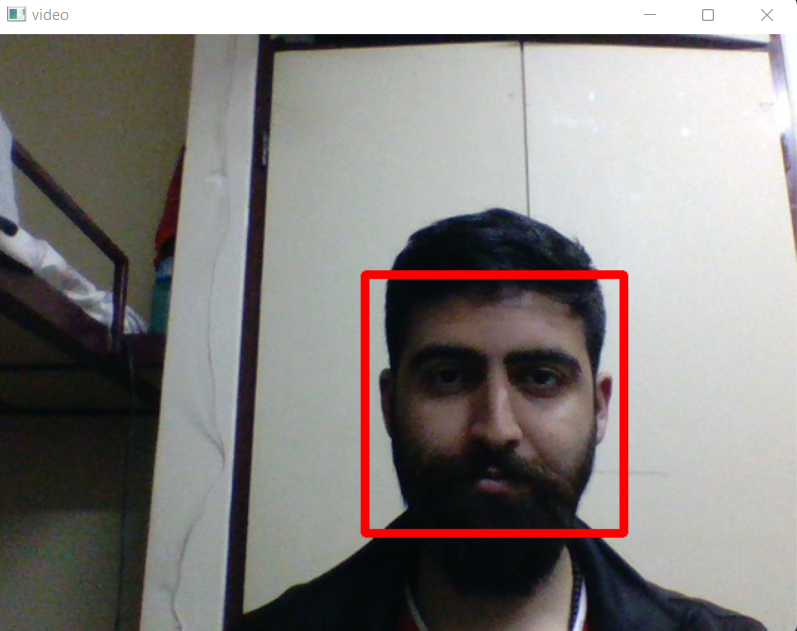
\includegraphics[width=0.5\textwidth]{images/face_detect}
	\caption{خروجی فاز تشخیص چهره}
	\label{تشخیص‌چهره}
\end{figure}

پس از تشخیص چهره نوبت به شناسایی آن می‌رسد. این کار به کمک شبکه عمیق از پیش آموزش دیده شده انجام می‌شود. « شکل \ref{شناسایی‌چهره} »
\begin{figure}[h]
	\centering
	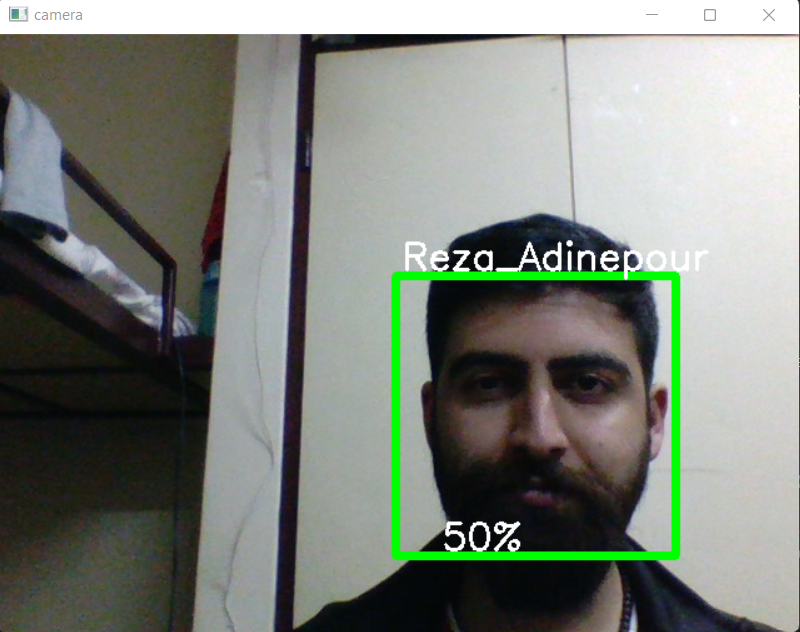
\includegraphics[width=0.5\textwidth]{images/face_recog}
	\caption{خروجی فاز شناسایی چهره}
	\label{شناسایی‌چهره}
\end{figure}

\newpage

برای انجام این مراحل یک رابط کاربری\footnote{\lr{User Interface}} به صورت زیر هم طراحی شده است. « شکل \ref{رابط کاربری} »
\begin{figure}[h]
	\centering
	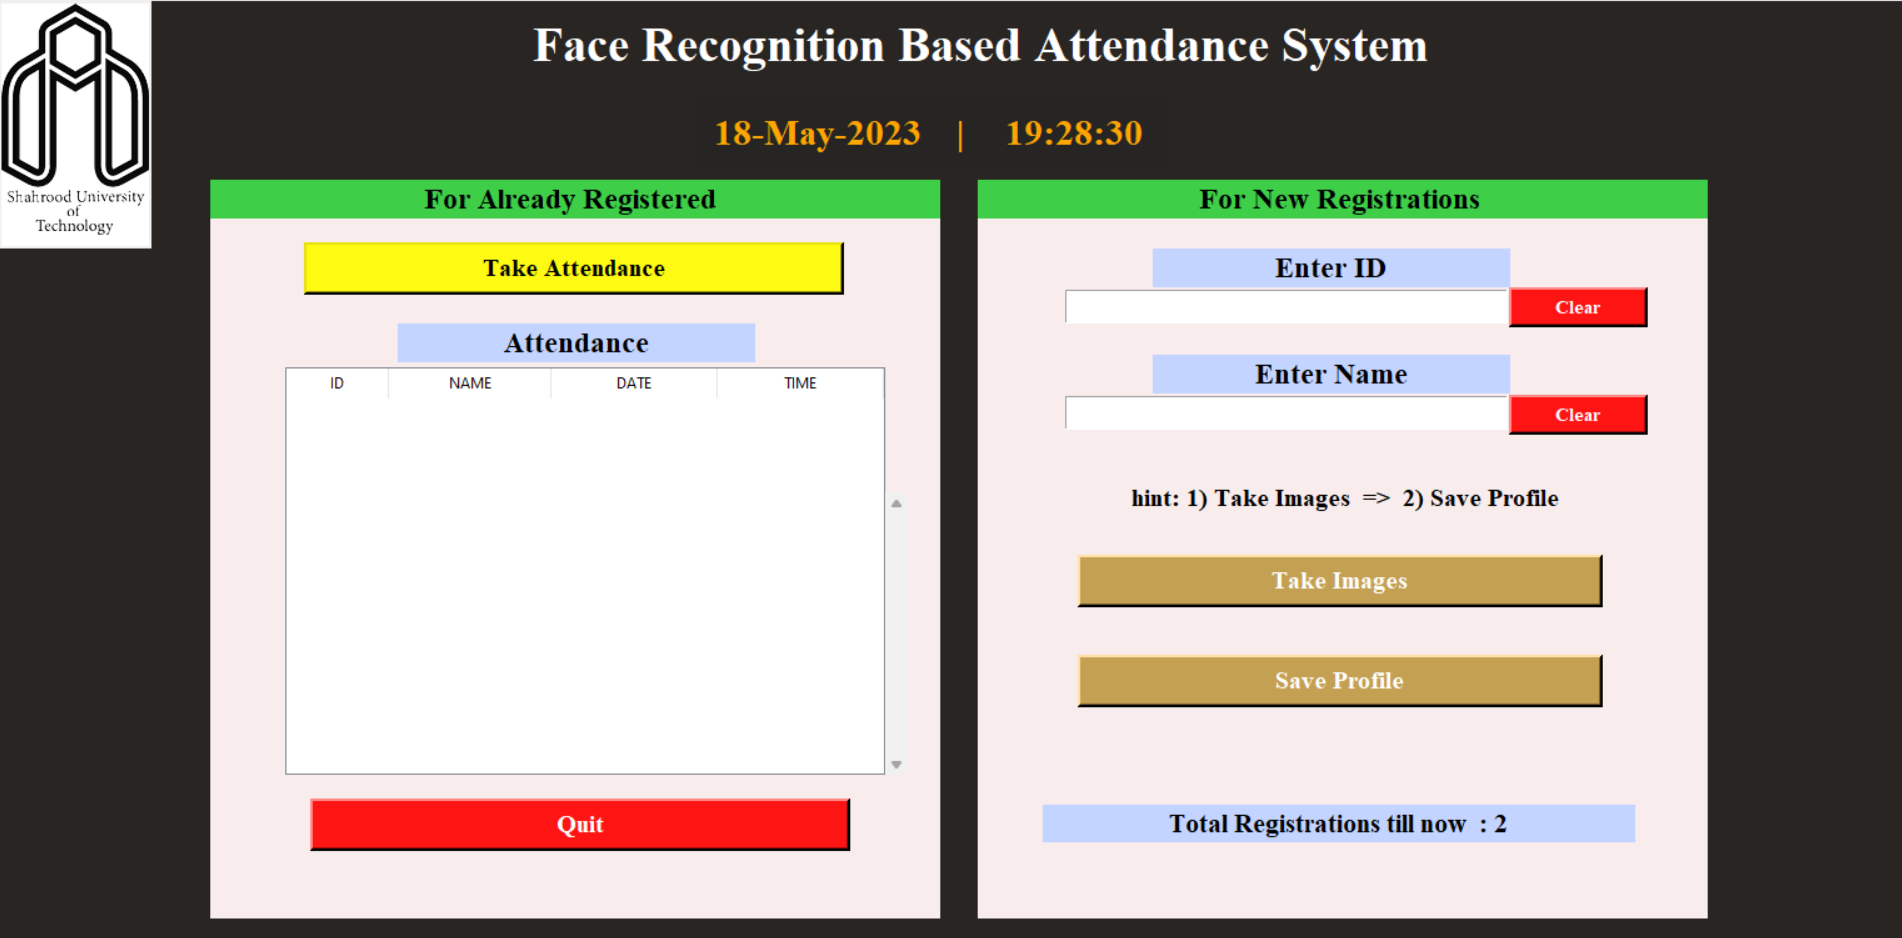
\includegraphics[width=0.9\textwidth]{images/user_interface}
	\caption{رابط کاربری سیستم}
	\label{رابط کاربری}
\end{figure}

\newpage

تمامی مراحل توضیحات داده شده در قسمت‌های قبل، بر روی مینی‌کامپیوتر \lr{Odroid-XU4} پیاده‌سازی شده است. « شکل \ref{اودروید} »
\begin{figure}[h]
	\centering
	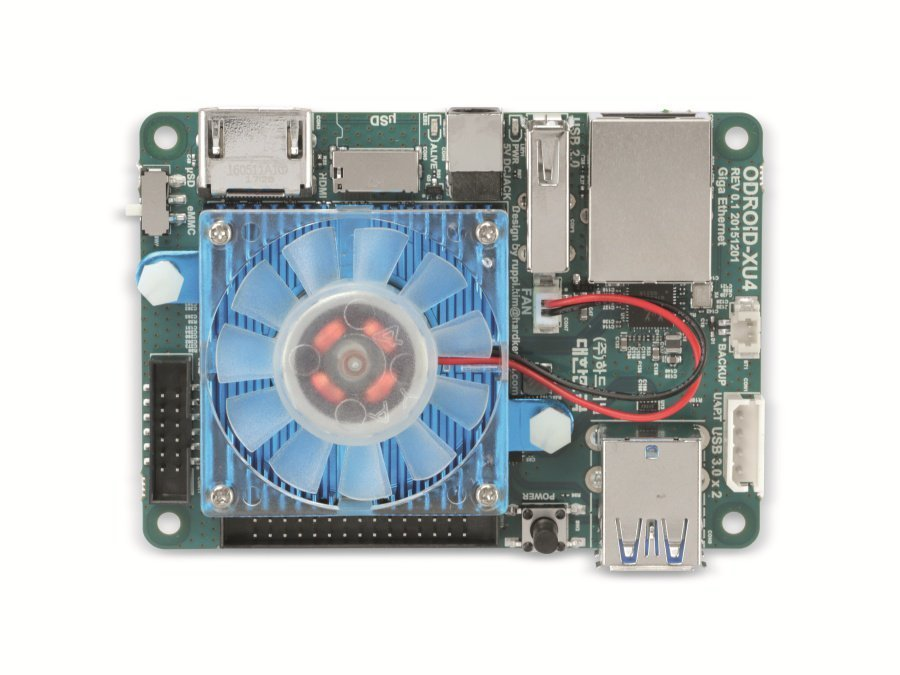
\includegraphics[width=1\textwidth]{images/odroid}
	\caption{سخت‌افزار استفاده شده}
	\label{اودروید}
\end{figure}

\end{document}